\sub{User Perspektive}
Die folgende \hyperref[tab:user]{Tabelle} zeigt die Software-Anforderungen an eine offlinefähige Kontaktliste aus der NutzerInnenperspektive.
\begin{longtable}[c]{@{}
>{\columncolor[HTML]{CFFCC2}}l ll@{}}
\toprule
    \multicolumn{1}{p{0.15\textwidth}}{\cellcolor[HTML]{cffcc2}\textbf{ID}}
    & \multicolumn{1}{p{0.85\textwidth}}{\cellcolor[HTML]{cffcc2}\textbf{Anforderung aus Userperspektive}}\\ \hline
\endfirsthead
%
\endhead
%
  \multicolumn{1}{l}{\cellcolor[HTML]{cffcc2}\textbf{User-Story 1}} &
  \multicolumn{1}{p{0.85\textwidth}}
  {Ich als NutzerIn möchte die Anwendung immer und überall, auch ohne Internetzugang zu nutzen.}\\
  \midrule
  %
  \multicolumn{1}{l}{\cellcolor[HTML]{cffcc2}\textbf{User-Story 2}} &
  \multicolumn{1}{p{0.85\textwidth}}
  {Ich als Nutzerin möchte, dass die Kontaktliste schnell und effizient geladen wird, um Zeit zu sparen.}\\
  \midrule
  %
  \multicolumn{1}{l}{\cellcolor[HTML]{cffcc2}\textbf{User-Story 3}} &
  \multicolumn{1}{p{0.85\textwidth}}
  {Ich als NutzerIn möchte jeden Kontakteintrag finden, um zu wissen ob ich ihn schon gespeichert habe.}\\
  \midrule
  %
  \multicolumn{1}{l}{\cellcolor[HTML]{cffcc2}\textbf{User-Story 4}} &
  \multicolumn{1}{p{0.85\textwidth}}
  {Ich als NutzerIn möchte Einträge immer und überall, auch ohne Internetzugang, erstellen, editieren oder löschen können, um meine Liste zu verwalten.}\\
  \midrule
  %
  \multicolumn{1}{l}{\cellcolor[HTML]{cffcc2}\textbf{User-Story 5}} &
  \multicolumn{1}{p{0.85\textwidth}}
  {Ich als NutzerIn möchte keine in der Anwendung gespeicherten Daten verlieren.}\\
  % end
  \bottomrule \cellcolor[HTML]{FFFFFF}
  \vspace{0.1cm}\\
  \noalign{\hspace{0.0525\textwidth}\grayRule}
  \caption{Anforderungen aus Userperspektive}
  \label{tab:user}\\
\end{longtable}

% Das in Abbildung \ref{fig:uc} gezeigte Use-Case-Diagramm veranschaulicht die in der obigen Tabelle \ref{tab:uc} aufgeführten Anwendungsfälle.
% \begin{figure}[H]
%     \centering
%     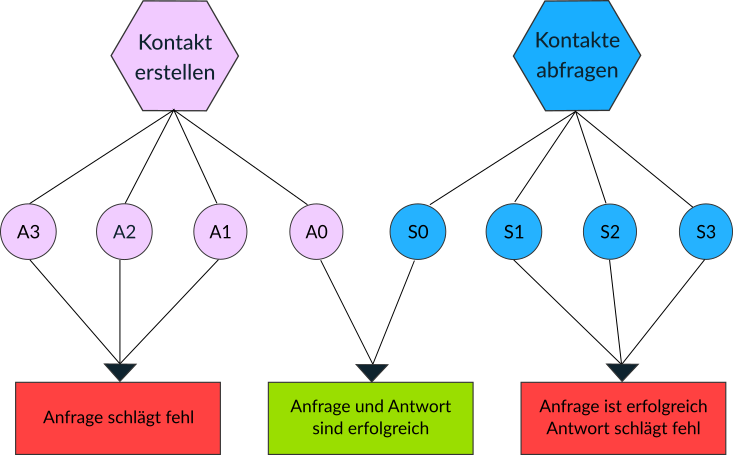
\includegraphics[width=0.4\textwidth]{Szenarien}
%     \grayRule
%     \caption[Use-Case Diagramm]{Platzhalter für US-Diagramm}
%     \label{fig:uc}
% \end{figure}